%!TEX root = thesis.tex

\chapter{Monitoring Timing Constraints on possibly infinite Streams}
\label{chapter-monitorability}
	The goal of this thesis is to implement online monitors for the TADL2 Timing Constraints on possibly infinite streams. An online monitor checks the current execution of a system, parallel to its execution. Because every computing system has finite memory resources and the online monitor should be able to process more events than occurs in the stream in a specific amount time, not every property can be monitored in an online monitoring setting. In this chapter, the term of \emph{Finite Monitorability} will be introduced, which ensures that monitoring a property on infinite streams is possible with finite memory resources and finite time resources per event. As introduction into the setting, some related work will be described, inter alia \emph{TeSSLa}, the programming language which is used for the implementation.

\section{Related Work}

	\subsubsection{Runtime Verification}
		As monitoring plays a major role in runtime verification, a short overview of this will be given. The definitions of \cite{RuntimeVerification} are used, in which \emph{Runtime Verification} is a technique that can detect deviations between the run of a system and its formal specification by checking correctness properties. A \emph{run}, which might also be called \emph{trace}, is sequence of the system states, which might be infinite and an \emph{execution} is an finite prefix of this run. A \emph{monitor} reads the trace and decides, whether it fulfills the correctness properties or violates them.\\
		A distinction is made between \emph{offline} and \emph{online} monitoring. Offline monitoring is using a stored trace, that has been recorded before. Therefore, the complete trace (or the complete part of the trace, that should be analyzed) is known in the analysis. Online monitoring checks the properties, while the system is running, which means that the analysis must be done incrementally on a growing prefix of the trace. Because of memory and time limitations, not all previous states can be read again in online monitoring, more detailed contemplations on the limitations of online monitors will be given in in this chapter.

	\subsubsection{TeSSLa}
		TeSSLa (\textbf{Te}mporal \textbf{S}tream-based \textbf{S}pecification \textbf{La}nguage) \cite{TeSSLa1} is a specification language build for stream Stream Runtime Verification. In TeSSLa, all streams in one specification must have a common global clock, but events or changes in a signal may occur in streams irregularly, independent of events in other streams. The verified streams are either considered as signal, which remain unchanged for certain amount of time (called \textit{piece wise constant signals}), or they are \textit{event streams}, in which each event consists of a timestamp and a data value. Both variants can be transferred into each other, like described in \cite{TeSSLa1}. A formal definition of the TeSSLa language core can be found in \cite{TeSSLa2}, a short overview of the formal definition of event streams will be given next.\\
		An event stream is defined over a time domain $\mathbb{T}$ and a data domain $\mathbb{D}$ and is an possibly infinite sequence $s=a_0a_1...\in\mathcal{S}_D=(\mathbb{T}\cdot\mathbb{D})^\omega\cup(\mathbb{T}\cdot\mathbb{D})^+\cup(\mathbb{T}\cdot\mathbb{D})^*\cdot(\mathbb{T}_\infty\cup\mathbb{T}\cdot\{\bot\})$ where $a_{2i} < a_{2(i+1)}$ for all $i$ with $0 < 2(i + 1) < |s|$ ($0 < 2(i + 1) < \infty$ if the sequence is infinite). While the data domain $\mathbb{D}$ can be bounded (e.g. boolean or integer) or unbounded (e.g. maps or lists), the time domain $\mathbb{T}$ is a \emph{totally ordered semi-ring} $(\mathbb{T}, 0, 1, +, *, \leq)$, that is not negative.\\
		In TeSSLa, computations are done, when new events are arriving. Based on the specification, output streams are generated with events on the same timestamps as the used input streams, but filtering is possible, where not all input events produce output events. With the \emph{delay}-operator, it is possible to create new timestamps. In a memory perspective, streams are not understood as event streams, but as \textit{piece wise constant signals}. Only the timestamp and the data value of the youngest event can be directly accessed. This event is available until the next event of this stream occurs. With the use of the \textit{last}-operator, which can be used recursively, the data value of the previous event can be accessed. Another important operator is the \textit{lift}-operator, which applies a function on data values (for example the $+$ operator) on the data value of every event of one or more streams and creates a new stream with events at the same timestamps and the results of the function as data values.
		
	\subsubsection{LOLA-Efficient Monitorable}
		\cite{LOLA} introduces \textit{LOLA}, a specification language for the observation of synchronous event streams, comparable to TeSSLa.The paper also defines the term of \textit{Efficiently Monitorable Specifications}, which describes that the worst case memory requirement of a LOLA Specification is independent of the length of the observed trace.
	
	
	\subsubsection{Deterministic Finite State Transducer\cite{Berstel1979}}
		A \textit{Deterministic Finite State Transducer}(DFST) is a 5-Tuple $(\Sigma, \Gamma, Q, q_0, \delta)$, where
		\begin{itemize}
			\item
				$\Sigma$ is an input alphabet
			\item
				$\Gamma$ is an output alphabet
			\item
				$Q$ is a finite set of states, with initial state $q_0$
			\item
				$\delta:Q\times\Sigma\rightarrow Q\times\Gamma$ is a state transition function 
		\end{itemize}
		DFSTs are similar to deterministic finite automata, with two major differences. First, the transition function outputs a symbol of $\Gamma$ at every transition and second, the DFST is not accepting, it only \textit{transduces} an input word.
		
	\subsubsection{Timed Deterministic Finite State Transducer}
		\textit{Timed Deterministic Finite State Transducer}(TDFST) are an extension of DFSTs. They are defined as 6-Tuple $(\Sigma, \Gamma, Q, q_0, C, \delta)$, where
		\begin{itemize}
			\item
				$\Sigma$ is an input alphabet
			\item
				$\Gamma$ is an output alphabet
			\item
				$Q$ is a finite set of states, with initial state $q_0$
			\item
				$C$ is a set of clocks
			\item
				$\delta:Q\times\Sigma\times\Theta(C)\rightarrow Q\times 2^C\times\Gamma$ is a state transition function 
		\end{itemize}
		Additional to the input symbols and the current state, the state transition function of TDFSTs takes a set of clock constraints into account when defining the next state of the transducer.
	
\section{Monitorability}
	In this section, the term \textit{Finite Monitorability} is introduced. It represents a stricter alternative to \textit{Efficiently Monitorable Specifications} mentioned above, by also restricting the allowed run time per event. \textit{Finite Monitorability} ensures, that the worst case memory consumption of a monitor is independent of the input events, consequently can every finite monitorable property be monitored with a efficient monitorable LOLA specification. 
	\subsubsection{Preliminary - Timestamps}
		\label{monitorability_timestamps}
		As we consider possibly infinite streams, the time value of events can also grow into infinity. This is problematic, because it leads to infinite memory and runtime requirements, which cannot be met, especially not in the context of online monitoring. Therefore, the time domain $\mathbb{T}$ is restricted by the following constraints:
		\begin{itemize}
			\item
				$\mathbb{T}$ must be discrete.
			\item
				The first used timestamp has the value $t_0=0$
			\item
				All used timestamps must be smaller than $t_{max}$.\\
				$t_{max}$ must be big enough, so it is not reached in practical use \footnote{for example, a 64-bit unsigned integer variable is enough, to cover nanoseconds for 584.55 years}.
			\item
				The distance between two subsequent time values is small enough to observe the wanted property.
		\end{itemize}

	\subsubsection{Finite Monitorability}
		The concept behind the definition of \textit{finite monitorability} is, that a monitor for event streams is defined by three parts, first the state transition function, a state defining the memory of the monitor and an output function. At each timestamp containing input events, the new state is created by applying the state transition function to the previous state and the input events of the current timestamp. The output function is applied to the new state and the previous output and evaluates, whether the specification is met until this timestamp.\\
		All following definitions of streams and functions follow the syntax and semantic from \cite{TeSSLa2}. The left half of figure~\ref{fig:OverviewMonitorability} visualizes the definitions, which will be done now.
		\begin{itemize}
			\item{\textbf{Input Streams}}\\
				Let $S_1, S_2, ..., S_n$ be the input streams with\\
				$\forall i:$ $S_i=(\mathbb{T}\cdot \mathbb{D}_i)^\omega\cup(\mathbb{T}\cdot \mathbb{D}_i)^+\cup(\mathbb{T}\cdot \mathbb{D}_i)^*\cdot(\mathbb{T}_\infty\cup\mathbb{T}\cdot\{\bot\})$\\
				All types $D_i$ have a finite size.
			\item{\textbf{State Stream}}\\
				\label{monitorability_state}
				Let $S_{state}$ with $S_{state}= (\mathbb{T}\cdot \mathbb{D}_{state})^+\cup(\mathbb{T}\cdot \mathbb{D}_{state})^*$
				be a state stream, where $\mathbb{D}_{state}$ has a constant worst case memory requirement.\\
				Further let $f: S_1 \times S_2 \times ... \times S_n \times S_{state}\rightarrow S_{state}\times \mathbb{T}$ be a state transition function, which defines the state stream in an incremental fashion:\newpage
				\begin{math}
					\forall t\in \mathbb T \exists i\in \{1,2,...,n\}: S_i(t)\in\mathbb D_i\\
					\rightarrow S_{state}(t)= f(S_1(t), S_2(t), ..., S_n(t), last(S_{state}, merge(S_1, S_2, ..., S_n))(t))
				\end{math}\\
				The runtime of $f$ is in $\mathcal{O}(1)$.
			\item{\textbf{Output Stream}}\\
				Let $S_{output}= (\mathbb{T}\cdot \{true_{until}, false\})^+\cup(\mathbb{T}\cdot \{true_{until}, false\})^*$\\
				be the output stream, which is defined via a function\\
				$g: \mathbb{D}_{state}\times\{true_{until}, false\}\times \mathbb{T}\rightarrow \{true_{until}, false\}\times \mathbb{T}$\\
				The runtime of $g$ is in $\mathcal{O}(1)$.
			\item{\textbf{Evaluation}}
				A property of a set of streams is called \emph{Finite Monitorable}, if a state transition function $f$, a type $\mathbb{D}_{state}$ and a output function $g$ exist, which fulfill the characteristics called above, and which outputs $true_{until}$, as long as the property is fulfilled and $false$, in any other case. It should be noted that these definitions are \emph{timestamp conservative}, because no new timestamps are created.
			\item{\textbf{Equivalences}}\\
				The combination of a finite state and state transition function is equivalent to a Deterministic Finite State Transducer(DFST), where
				\begin{itemize}
					\item
						$Q=\mathbb{D}_{state}$ is the finite set of possible states with initial state $q_0$
					\item
						$\Sigma=((\mathbb{D}_1\times \mathbb{T}),...,(\mathbb{D}_n\times \mathbb{T}))$ the input alphabet
					\item
						$\Gamma = \mathbb D_{state}$ is the output alphabet and
					\item
						$\delta: Q\times \Sigma\rightarrow Q\times\Gamma$ is the transition function.
				\end{itemize}
				The definition of the output function $g: \mathbb{D}_{state}\times\{true_{until}, false\}\times \mathbb{T}\rightarrow \{true_{until}, false\}\times \mathbb{T}$ is the same as described above.\\
				It should be noted that the function $g$ could also be included into the DFST, which represents the state and the state transition function of the monitor without changing the expressiveness. This is not done to keep analogies to the following definition.
		\end{itemize}
	
	\begin{figure}
		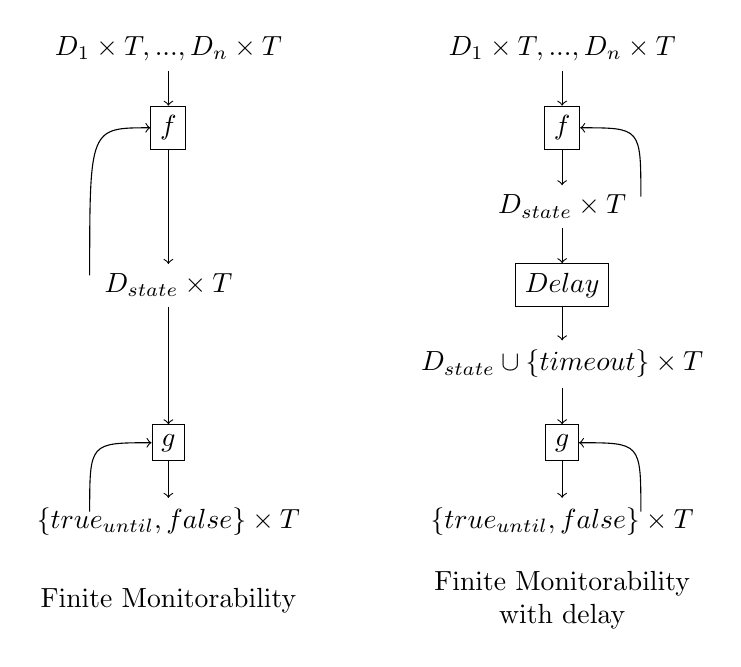
\begin{tikzpicture}
			\node[] (inputRight){$\mathbb{D}_1\times\mathbb{T}, ..., \mathbb{D}_n\times\mathbb{T}$};
			\node[draw, below of=inputRight] (fRight){$f$};
			\node[below of=fRight] (stateRight){$\mathbb{D}_{state}\times\mathbb{T}$};
			\node[draw, below of=stateRight] (delayRight){$Delay$};
			\node[below of=delayRight] (stateDelayRight){$\mathbb{D}_{state}\cup\{timeout\}\times\mathbb{T}$};
			\node[draw, below of=stateDelayRight] (gRight){$g$};
			\node[below of=gRight] (outputRight){$\{true_{until}, false\}\times\mathbb{T}$};
			
			\draw[->] (inputRight) -- (fRight);
			
			\node[right of = stateRight] (ha){};
			\node[right of = fRight] (hb){};
			\draw[->] (ha)  .. controls (hb) .. (fRight);
			
			\node[right of = outputRight] (hg){};
			\node[right of = gRight] (hh){};
			\draw[->] (hg)  .. controls (hh) .. (gRight);
			
			\draw[->] (fRight) -- (stateRight);
			\draw[->] (stateRight) -- (delayRight);
			\draw[->] (delayRight) -- (stateDelayRight);
			\draw[->] (stateDelayRight) -- (gRight);
			\draw[->] (gRight) -- (outputRight);
			\node [below of=outputRight, align=center] (h0){Finite Monitorability\\with delay};
			
			
			\node[left of = inputRight] (h1){};
			\node[left of = h1] (h2){};
			\node[left of = h2] (h3){};
			\node[left of = h3] (h4){};
			
			\node[left of = h4] (inputLeft){$\mathbb{D}_1\times\mathbb{T}, ..., \mathbb{D}_n\times\mathbb{T}$};
			\node[draw, below of=inputLeft] (fLeft){$f$};
			\node[below of = fLeft] (h5){};
			\node[below of=h5] (stateLeft){$\mathbb{D}_{state}\times\mathbb{T}$};
			\node[, below of=stateLeft] (delayLeft){};
			\node[draw, below of=delayLeft] (gLeft){$g$};
			\node[below of=gLeft] (outputLeft){$\{true_{until}, false\}\times\mathbb{T}$};
			\draw[->] (inputLeft) -- (fLeft);
			\draw[->] (fLeft) -- (stateLeft);
			\draw[->] (stateLeft) -- (gLeft);
			\draw[->] (gLeft) -- (outputLeft);
			
			\node[left of = stateLeft] (hc){};
			\node[left of = fLeft] (hd){};
			\draw[->] (hc)  .. controls (hd) .. (fLeft);
			
			\node[left of = outputLeft] (he){};
			\node[left of = gLeft] (hf){};
			\draw[->] (he)  .. controls (hf) .. (gLeft);
			
			\node [below of=outputLeft] {Finite Monitorability};
		\end{tikzpicture}
		\centering
		\caption{Overview Finite Monitorability - with or without \emph{delay}}
		\label{fig:OverviewMonitorability}
	\end{figure}
			
	\subsubsection{Finite Monitorability with Delay}
		Most of the TADL2 constraints can not be monitored in a \emph{timestamp conservative} way. For example, the \emph{RepeatConstraint} with the attributes $lower=upper=4$ and $span=1$ expects subsequent events to have a time distance of $4$. If one event is missing, the output of a timestamp conservative monitor would remain $true_{until}$, until the next input event arrives. Therefore, the monitor cannot not check the constraint correctly. Because of this problem, the definition of \emph{Finite Monitorability} is expanded by the ability of introducing new timestamps. To ensure the finiteness of the monitor, only one new timestamp can be introduced. The following definitions are visualized in the right half of figure~\ref{fig:OverviewMonitorability}.
		\begin{itemize}
			\item{\textbf{Input Streams}}\\
				The definition of the input streams are unchanged.
			\item{\textbf{State Stream}}
				The function $f$ remains unchanged, but the state stream $S_{state}$ is expanded by an \emph{timeout} value, which is inserted after a specific period of time, in which no input event has arrived. Like before, the runtime of $f$ is in $\mathcal{O}(1)$.
			\item{\textbf{Delay}}\\
				\label{DelayGenerator}
				A \emph{Delay Generator} is inserted into the definition. It has two tasks, first it copies each input it gets from the state transition function $f$ to its output. At the timestamp where an input is copied, a timer, which length depends on the state of the monitor, is started. If the next input comes before the timer runs out, the timer is resetted and started again. If the timer runs out, the Delay Generator outputs the $timeout$ signal, which is repeated at every following input. After the timer has run out once, it is not started again. The calculation of the needed delay is in $\mathcal{O}(1)$ in terms of time.
			\item{\textbf{Output Stream}}\\
				The input of the output function $g$ is expanded by the $timeout$ value:\\
				$g: (\mathbb{D}_{state}\cup\{timeout\})\times \mathbb{T}\rightarrow \{true_{until}, false\}\times \mathbb{T}$\\ 
				Obviously, $g$ always outputs false, if the functions receives the $timeout$ value. The definition of the output stream $S_{output}$ remains unchanged.
			\item{\textbf{Evaluation}}\\
				A property of a set of streams is called \emph{Finite Monitorable with Delay}, if a function $f$, a type $\mathbb{D}_{state}$, a delay generator and a function $g$ exist, which fulfill the characteristics called above, and which outputs $true_{until}$, as long as the property is fulfilled and $false$, in any other case.
			\item{\textbf{Equivalences}}
				Similar to \textit{Finite Monitorability} (without Delay), equivalences to finite state machines can be worked out. Like before, the combination of a finite state and state transition function is equivalent to a Deterministic Finite State Transducer(DFST), where
				\begin{itemize}
					\item
					$Q=\mathbb{D}_{state}$ is the finite set of possible states with initial state $q_0$
					\item
					$\Sigma=((\mathbb{D}_1\times \mathbb{T}),...,(\mathbb{D}_n\times \mathbb{T}))$ the input alphabet
					\item
					$\Gamma = \mathbb D_{state}$ is the output alphabet and
					\item
					$\delta: Q\times \Sigma\rightarrow Q\times\Gamma$ is the transition function.
				\end{itemize}
				The \textit{Delay Generator} is equivalent to an extended version of \textit{Timed Deterministic Finite State Transducer}, which allows $\epsilon$-transitions, which are guarded by a clock constraint, but do not require an input symbol to perform a state transition. This special form of TDFSTs will be defined next.\\ \\
				Let $tmr:\mathbb{D}_{state}\rightarrow\mathbb{T}$ be a function that determines the required delay for every possible state of the monitor. Let further
				\begin{itemize}
					\item
						$Q = \{q_{start}, q_{timeout}\}\cup\{q_{wait,i} | \forall i\in \mathbb{D}_{state}\}$ be a finite set of states with initial state $q_{start}$
					\item
						$\Sigma = \mathbb D_{state}$ be an input alphabet
					\item
						$\Gamma = \mathbb D_{state} \cup \{timeout\}$ be an output alphabet
					\item
						$C=\{c\}$ be a set of exactly one clock and
					\item
						$\delta:Q\times(\Sigma\cup\{\epsilon\})\times\Theta(C)\rightarrow Q\times 2^C\times\Gamma$ a state transition function. $\delta$ is defined as:
						\begin{align}
							\forall i\in \mathbb{D}_{state}:\delta(q_{start}, i, \emptyset) &= (q_{wait,i}, \{c\}, i)\\
							\forall i, i'\in \mathbb{D}_{state}:\delta(q_{wait, i'}, i, \{c < tmr(i')\}) &= (q_{wait,i}, \{c\}, i)\\
							\forall i \in \mathbb{D}_{state}:\delta(q_{wait, i}, \epsilon, \{c < tmr(i)\}) &= (q_{timeout}, \emptyset, timeout)\\
							\forall i \in \mathbb{D}_{state}:\delta(q_{timeout}, i, \emptyset) &= (q_{timeout}, \emptyset, timeout)
						\end{align}
				\end{itemize}
				This definition is visualized in figure~\ref{fig:DelayGenerator}. On the left side is the initial state. The first input leads to a transition to the wait state of the corresponding input state. The clock $c$ is resetted in this transition. In the middle column of the figure are the wait states, one for each possible state of the monitor. $|\mathbb{D}_I|+1$ transitions leave each wait state, one is the $\epsilon$-transition introduced above, which is constrained in a way, that the value of clock $c$ must be equal or greater than the corresponding delay time. This $\epsilon$-transition leads to $q_timeout$ and outputs the \textit{timeout} symbol. Every other transition leaving the waiting states are done at input symbols, while the value of clock $c$ is less than the corresponding delay time. In these transitions, the input symbol $d_i$ is used as output and clock $c$ is resetted. In the output state, each input symbol leads to a repetition of the \textit{timeout} symbol.
				
				
				
				Like before, the output function is defined as $g: (\mathbb{D}_{state}\cup\{timeout\})\times \mathbb{T}\rightarrow \{true_{until}, false\}\times \mathbb{T}$.
		\end{itemize}

	\begin{figure}
		\begin{tikzpicture}[state/.style={draw, circle,minimum size=1.5cm, node distance=3cm}]
			\node[state, initial] at (0,0)(qstart)  {$q_{start}$};
			
			\node[state] at(3,2) (qwait1){$q_{wait,d_1}$};
			\node[]at (3,0) (qWaitBla){...};
			\node[state]at(3,-2) (qwaitn){$q_{wait,d_n}$};
			
			\node[state] at(6,0) (qTimeOut){$q_{timeout}$};
			
			\path[->] 	(qstart) edge node[left, near end]{$(d_1, \emptyset, \{c\}, d_1)$} (qwait1)
						(qstart) edge node[left, near end]{$(d_n, \emptyset, \{c\}, d_n)$} (qwaitn)
						(qwait1) edge node[right]{$(\epsilon, \{c \geq tmr(d_1)\}, \emptyset, timeout)$} (qTimeOut)
						(qwaitn) edge node[right]{$(\epsilon, \{c \geq tmr(d_n)\}, \emptyset, timeout)$} (qTimeOut)
						(qwait1) edge[loop above] node{$(d_1, \{c < tmr(d_1)\}, \{c\}, d_1)$}()
						(qwait1) edge[bend left] node[right, near end]{A}(qwaitn)
						(qwaitn) edge[bend left] node[right, near end]{B}(qwait1)
						(qwaitn) edge[loop below] node{$(d_n, \{c < tmr(d_n)\}, \{c\}, d_n)$}()
						(qTimeOut) edge[loop right] node{$\forall d_i \in \mathbb{D}_I:(d_i, \emptyset, \emptyset, timeout)$}();
						
			
		\end{tikzpicture}
		\label{fig:DelayGenerator}
		\caption{Visualization of the Delay Generator. Description A means $(d_n, \{c < tmr(d_1)\}, \{c\}, d_n)$ and description B means $(d_1, \{c < tmr(d_n)\}, \{c\}, d_1)$.}
	\end{figure}
			

			
	\subsubsection{Non-Finite Monitorability}
		Not all TADL2 constraints are finite monitorable, because they may require memory or time resources, which size is not independent from the events of the observed trace. This makes correct online monitoring of these constraints impossible for arbitrary traces, because a machine with infinite resources does not exist. In a practical view, many of these problems are solved by using a system with finite memory, with the hope that its finite memory would be enough, to cover the inputs of the ''real world''. In these cases, a distinction is useful, as the memory requirements of some properties grow continuously with every input event, and other constraints only require infinite resources in worst case scenarios. The ones with continuous requirement growth will be called \emph{always Non-Finite Monitorable} and the others \emph{worst case Non-Finite Monitorable} in the following.\\
		Obviously, the constraints with continuous resource requirement growth cannot be monitored infinitely, but the constraints, that only need infinite resources, can be monitored in many cases.

	 